\section{Theoretical framework}
\label{sec:Theory}
%Zijn er knowlage/algorithme `gaps'
%wetenschappelijke bijdrage van dit project
%\subsection{Image recognition}
%\label{sec:Theory-CV}
The history of Image Recognition begins as a summer school of Stanford.
As was the case in that age, Artificial Intelligence made some wild assumptions on the reachability of their projects. \citeneed
The recent developments show how mistaken they were.

Through the years multiple algorithms have been made to accomplice Computer Vision.
The model used to describe images has been a grid with a value (the pixels).
This results in a multidimensional function, on which several linear and geometric algebra algorithms can be used on.
Usually three steps are taken to identify an image.
First using the gradient in images, key-points of the image are identified.
Thereafter, these key-points are used to construct features or models, describing the image.
Finally these models are tested against a classifier. \citeneed

%The Convolutional Neural Network uses the same kind of steps.
%However, part of the models and representations of the images are not made by humans, as is the case in most other algorithms, but learnt by the network itself.

\subsection{Image representations}
\label{sec:Theory-image}
As stated above, local image gradients are used to make models on which classifiers can be trained.
Several techniques exists that extract features from the image and make a descriptor.
A wildly used technique for extracting the features is a `Bag of Features'; the frequency of the features result in a multidimensional vector of the size of the number of features.
From the data-points representing the images, a classifier can be trained. \citeneed

Another possibility is using a Convolutional Neural Network.
The CNN does a similar trick with the features.
However, it also constructs the features itself from the image-data and has the possibility to be used as a classifier.
In other words, a CNN can be used for each of the steps needed for classifying images.

The CNN technique is currently popular with image recognition tasks.
From large amounts of data, an accurate recognition system can be trained \citep{girshick2014rich}, \citep{razavian2014cnn}.

The biggest difference between `classical' imaging techniques --such as Bag of Features-- and Convolutional Neural Networks is the self-learning of the CNN.
The neurons of a CNN are trained on the data and construct their own representation that describes the images.
In contrary to classical techniques, from which the representations are constructed by humans that build the algorithms.

%\todo{structuur: -image representations(bow, cnn). -image classification (svm=meest voorkomend)}

%Eerdere bevindingen recognition %--/kleur
%Current image recognition and detection algorithms specialise on neural-nets... [oa citeren \citep{szeliski2010computer}] Current state-of-the-art results...
% Kriz, Hinton of LeCun was logischer geweest. Of naar de hele ImageNet 2014 competitie
%\subsection{CNN}
%\label{sec:Theory-CNN}
%What is CNN and how does it work... [oa citeren \citep{jia2014caffe}, \citep{razavian2014cnn}, \citep{girshick2014rich} ]
%...CNNs exist since the 1980's... mimic part of human brains...
%...layers of neurons... weights...
%==waarom CNNs zo goed werken lijken te voor image recognition en speech recognition tasks. 
%...since 2011 implementation for fast calculations on GPU...
%...high performance probably because of `learned' representations instead of `man-made'...

In the Machine Learning the Convolutional Neural Network (CNN) has existed for quite some time \citep{fukushima1980neocognition}.
However, due to computational complexity is was only recently that \citet{krizhevsky2012imagenet} showed an implementation to compute large CNNs.
\citeauthor{krizhevsky2012imagenet} shows how to implement a CNN on a computer's GPU that can work with the massive parallelism necessary to compute many layers of nodes.

Neural Networks consist of nodes, connected with weighted edges.
When data is presented to the input of the network, each node calculates with its input an output, which results in an output of the network.
When the output of the network is incorrect according to the label of the input, a backward calculation in the network is performed.
This calculation makes an adaptation to the weights in such a manner, that the network will output the correct label in the next run.

A CNN is a neural network that consists of several layers of nodes, with sometimes many millions of neurons.
Figure \ref{fig:cnn-alex} shows the layers of neurons the CNN used by \citeauthor{krizhevsky2012imagenet}.

\begin{figure}[h!tb]
\centering
\ifx\showfig\undefined
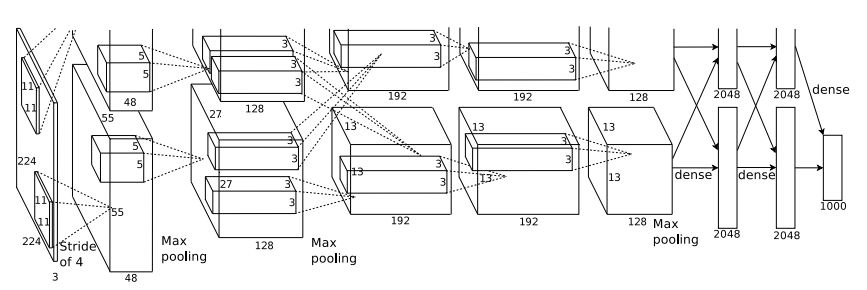
\includegraphics[keepaspectratio=true,width=\textwidth]{images/alexnet2012.png} \fi
\caption{Model of the layers of neurons in the CNN as used by \citet{krizhevsky2012imagenet}}
\label{fig:cnn-alex}
\end{figure}

Though a CNN can be used to classify a dataset of images, training such a network uses much computing power.
A pre-trained CNN has the weights of the neurons adapted to the dataset used for training.
This results in a network trained on other classes than used for this project.
However, a method that can be applied to work around this problem is inherent to the workings of a CNN.

%The dataset in this project is small with only 40k images.
%Therefore training a CNN will not be possible.
%However, because of the manner a CNN is build, it will not be necessary to fully train the network.

The bottom layers of a CNN trained on large image datasets detect basic visual concepts, for instance lines, corners and simple shapes.
Only higher in the network the concepts become more abstract and less local \citep{zeiler2014visualizing}.
Therefore, using the second-to-last layer of a pre-trained CNN an abstract representation of the image can be obtained.

This second-to-last layer can be represented as a multidimensional vector in a space the size of the number of abstract features.
As stated before, a feature-vector can be used to train a classifier.
Effectively, this project uses a pre-trained CNN as a feature extractor of an image to train an SVM classifier.

%--\subsection{Colour}
%--What is colour and why is it important... [oa citeren \citep{van2010evaluating}, \citep{ai2010color}]
%\subsection{Principal Component Analysis}
%\label{sec:Theory-PCA}
%\todo{Write this section (or delete it)}
\subsection{Image classification}
\label{sec:Theory-class}
Classifying feature-vectors has also several possible algorithms.
The Support Vector Machine (SVM) is one of the classification algorithms in Machine Learning that is wildly used in supervised image classification.
%In contrary to k-means cluster algorithm, an SVM uses labelled data to classify \citepos.
%An SVM also works better in high-dimensional data than a k-means clustering \citeneed.
%However, an SVM works best when no more than two classes need to be classified.

The SVM uses the data-points as vectors in a high dimensional space.
In this space, several Linear Algebra techniques are used to fit a hyperplane in this space, where the distance (i.e. a projection of the vector on the plane) of each data-point is maximised.
Figure \ref{fig:svm-fits} shows an example in 2D of possible manners to divide the data-points in the classes; the solid line shows a maximised classifier.
The SVM results in a classifier where the sign of the projection vector classifies the data-points (i.e. on which side of the plane the data-point is).

\begin{figure}[h!tb]
\centering
\ifx\showfig\undefined
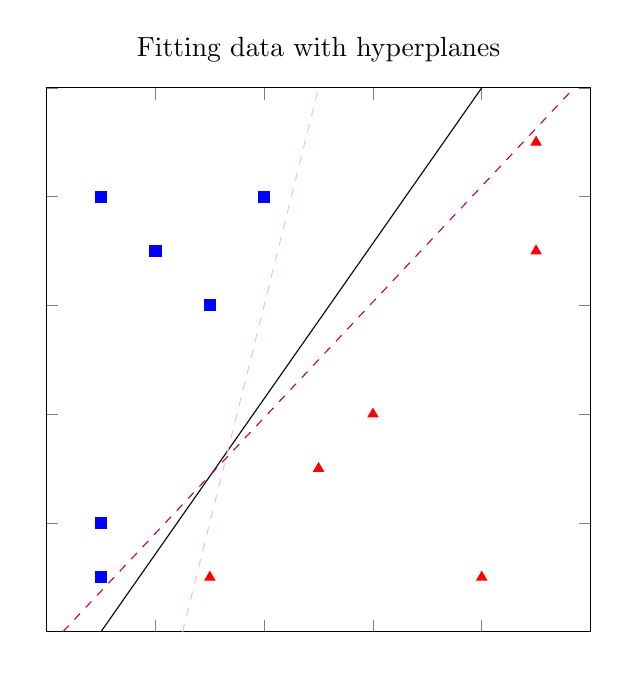
\begin{tikzpicture}
\begin{axis}[
    title={Fitting data with hyperplanes},
    width=.7\textwidth,
    height=.7\textwidth,
    xmin=0, xmax=10,
    ymin=0, ymax=10,
    yticklabels={,,},
    xticklabels={,,},
]
\addplot[
    color=blue,
    mark=square*,
    only marks,
    ]
    coordinates {
    (1,1) (1,2) (1,8) (2,7) (4,8) (3,6)
    };
\addplot[
    color=red,
    mark=triangle*,
    only marks
    ]
    coordinates {
    (3,1) (8,1) (5,3) (6,4) (9,7) (9,9)
    };
\addplot[
    color=black,
    ]
    coordinates{
    (1,0) (8,10)
    };
\addplot[
    color=pink, dashed
    ]
    coordinates{
    (2.5,0) (5,10)
    };
\addplot[
    color=purple, dashed
    ]
    coordinates{
    (0.3,0) (9.7,10)
    };
\end{axis}
\end{tikzpicture} \fi
\caption{Example of possible possible classifications in an algorithm. The dotted lines are a worse fit than the continuous one.}
\label{fig:svm-fits}
\end{figure}

The hyperplane that describes the classifier can be described by, besides linear, other, more complex, formulae.
However, these planes usually need more calculation time than a linear plane.
Figure \ref{fig:svm-planes} shows the three hyperplanes used in this project.
The data in these examples show the necessity of the different hyperplanes for different data.

\begin{figure}[h!tb]
\centering
\ifx\showfig\undefined
\centerline{
\begin{minipage}{1.3\textwidth}
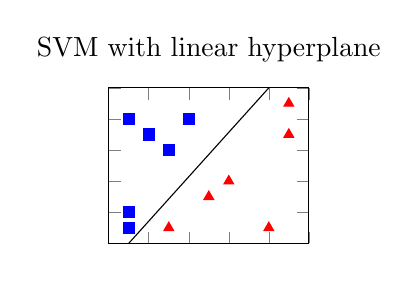
\begin{tikzpicture}
\begin{axis}[
    title={SVM with linear hyperplane},
    width=.34\textwidth,
    xmin=0, xmax=10,
    ymin=0, ymax=10,
    %xtick={0,...,10},
    yticklabels={,,},
    xticklabels={,,},
]
\addplot[
    color=blue,
    mark=square*,
    only marks,
    ]
    coordinates {
    (1,1) (1,2) (1,8) (2,7) (4,8) (3,6)
    };
\addplot[
    color=red,
    mark=triangle*,
    only marks
    ]
    coordinates {
    (3,1) (8,1) (5,3) (6,4) (9,7) (9,9)
    };
\addplot[
    color=black,
    ]
    coordinates{
    (1,0) (8,10)
    };
\end{axis}
\end{tikzpicture}
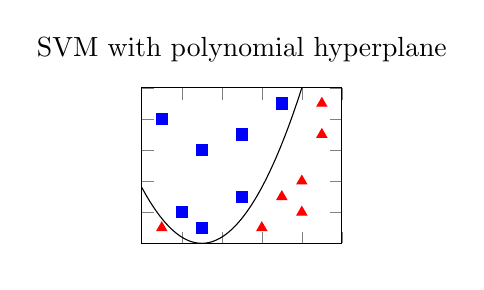
\begin{tikzpicture}
\begin{axis}[
    title={SVM with polynomial hyperplane},
    width=.34\textwidth,
    xmin=0, xmax=10,
    ymin=0, ymax=10,
    %xtick={0,...,10},
    yticklabels={,,},
    xticklabels={,,},
]
\addplot[
    color=blue,
    mark=square*,
    only marks,
    ]
    coordinates {
    (3,1) (2,2) (1,8) (5,7) (7,9) (3,6) (5,3)
    };
\addplot[
    color=red,
    mark=triangle*,
    only marks
    ]
    coordinates {
    (1,1) (6,1) (8,2) (7,3) (8,4) (9,7) (9,9)
    };
\addplot[
    color=black,
    domain=0:10,
    samples=100] (\x,{0.4*(\x-3)^2});
\end{axis}
\end{tikzpicture}
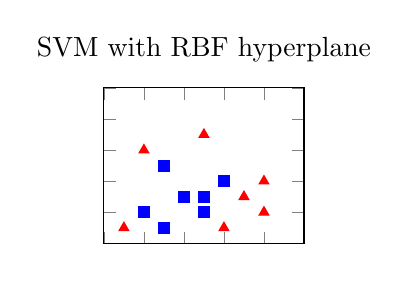
\begin{tikzpicture}
\begin{axis}[
    title={SVM with RBF hyperplane},
    width=.34\textwidth,
    xmin=0, xmax=10,
    ymin=0, ymax=10,
    %xtick={0,...,10},
    yticklabels={,,},
    xticklabels={,,},
]
\addplot[
    color=blue,
    mark=square*,
    only marks,
    ]
    coordinates {
    (3,1) (2,2) (5,2) (4,3) (6,4) (3,5) (5,3)
    };
\addplot[
    color=red,
    mark=triangle*,
    only marks
    ]
    coordinates {
    (1,1) (6,1) (8,2) (7,3) (8,4) (5,7) (2,6)
    };
\draw (axis cs:4,3) circle [black, radius=25];
\end{axis}
\end{tikzpicture}
\end{minipage}
} \fi
\caption{Examples of different hyperplanes of a two dimensional SVM }
\label{fig:svm-planes}
\end{figure}
%...classification in many dimensions... works by hyperplanes...
%--\subsection{Pre-process}
%--Before a CNN can be used, the imagedata needs to be pre-processed...
%--[oa citeren \citep{guo2010completed}, \citep{zhang2010local}]